\documentclass[class=jsarticle, crop=false, dvipdfmx, fleqn]{standalone}
%% preamble for Numerical-structure-analysis report

\input{/Users/User/Documents/Project/TeX/preamble/mypreamble}

%% titles
\title{先端データ解析論 レポート}
\author{37-196360 \quad 森田涼介}


%% setting for listings
\newtcbinputlisting[auto counter]{\reportlisting}[3][]{%
	listing file = {#3},
	listing options = {language=python, style=tcblatex, numbers=left, numberstyle=\tiny},
	listing only,
	breakable,
	toprule at break = 0mm,
	bottomrule at break = 0mm,
	left = 6mm,
	sharp corners,
	drop shadow,
	title = Listings \thetcbcounter : \texttt{#2},
	label = #1,
	}



%% title format
\usepackage{titlesec}
\titleformat{\section}{\LARGE}{宿題\thesection}{0zw}{}
\newcommand{\sectionbreak}{\clearpage}
\titleformat{\subsection}{\Large}{\Alph{subsection})}{0zw}{}

\begin{document}
\section{}

ガウスカーネルモデルに対して,
スパース回帰の交互方向乗数法による反復式を求め,
また適当なモデルに対してスパース回帰を実行する。


ガウスカーネルモデルは次のように表される。
\begin{align}
	& f_{\bm{\theta}} (\bm{x}) = \sum_{j=1}^{n} \theta_j K(\bm{x},\ \bm{x}_j) \\
	& K(\bm{x}, \bm{c}) = \exp(-\frac{||\bm{x} - \bm{c}||^2}{2 h^2})
\end{align}
このとき,L1正則化を用いた最小二乗誤差は,
\begin{align}
	& J(\bm{\theta}) = \frac{1}{2} ||\bm{K \theta} - \bm{y}||^2 + \lambda ||\bm{\theta}||_1 \\
	& \bm{K} =
		\begin{bmatrix}
			K(\bm{x}_1,\ \bm{x}_1) & \cdots & K(\bm{x}_1,\ \bm{x}_n) \\
			\vdots & \ddots & \vdots \\
			K(\bm{x}_n,\ \bm{x}_1) & \cdots & K(\bm{x}_n,\ \bm{x}_n)
		\end{bmatrix}
\end{align}
と表される。
このとき,最適なパラメータ\(\hat{\bm{\theta}}\)は次のように求まる。
\begin{equation}
	\hat{\bm{\theta}} = \arg\min_{\bm{\theta}} (J)
\end{equation}

\(J\)に最小を与える\(\bm{\theta}\)を,
以下の設定で交互方向乗数法を用いることで求める。
すなわち,
\begin{align}
	& \bm{\theta} - \bm{z} = \bm{0} \\
	& l(\bm{\theta}) = \frac{1}{2} ||\bm{K \theta} - \bm{y}||^2 \\
	& g(\bm{z}) = \lambda ||\bm{z}||_1
\end{align}
の下で,
\begin{align}
	\min_{\bm{\theta},\ \bm{z}}[l(\bm{\theta}) + g(\bm{z})]
\end{align}
を与える\(\bm{\theta},\ \bm{z}\)を求める。
このとき,拡張ラグランジュ関数は,
\begin{align}
	L(\bm{\theta},\ \bm{z},\ \bm{u})
		& = l(\bm{\theta}) + g(\bm{z}) + \bm{u}^\mathrm{T} (\bm{\theta} - \bm{z}) + \frac{1}{2} ||\bm{\theta} - \bm{z}||^2 \\
		& = \frac{1}{2} ||\bm{K \theta} - \bm{y}||^2 + \lambda ||\bm{z}||_1 + \bm{u}^\mathrm{T} (\bm{\theta} - \bm{z}) + \frac{1}{2} ||\bm{\theta} - \bm{z}||^2
\end{align}
であるから,\(\bm{K}\)は対称行列であることに注意すると,
\begin{align}
	\pdv{L}{\bm{\theta}}
		& = \bm{K}^2 \bm{\theta} - \bm{K y} + \bm{u} + (\bm{\theta} - \bm{z}) \\
		& = (\bm{K}^2 + \bm{I})\bm{\theta} - \bm{z} + \bm{u} - \bm{K y} \\
	\pdv{L}{\bm{z}}
		& = \lambda \pdv{||\bm{z}||_1}{\bm{z}} - \bm{u} + (\bm{z} - \bm{\theta}) \\
		& = \bm{z} - (\bm{\theta} + \bm{u} - \lambda \mathrm{sign}(\bm{z}))
\end{align}
となる。
よって,更新式は,
\begin{align}
	\bm{\theta}^{(t+1)}
		& = \arg\min_{\bm{\theta}} L(\bm{\theta},\ \bm{z}^{(t)},\ \bm{u}^{(t)}) \\
		& = (\bm{K}^2 + \bm{I})^{-1} (\bm{K y} + \bm{z}^{(t)} - \bm{u}^{(t)}) \\
	\bm{z}^{(t+1)}
		& = \max(\bm{0},\ \bm{\theta}^{(t+1)} + \bm{u}^{(t)} - \lambda) + \min(\bm{0},\ \bm{\theta}^{(t+1)} + \bm{u}^{(t)} + \lambda) \\
	\bm{u}^{(t+1)}
		& = \bm{u}^{(t)} + \bm{\theta}^{(t+1)} - \bm{z}^{(t+1)}
\end{align}
となる。

いま,真のデータが
\begin{equation}
	f(x) = \sin(\pi x) / (\pi x) + 0.1 x
		\quad (-3 \leq x < 3 )
\end{equation}
から生成されていて,
そのサンプルが50個ある場合を考える。
このデータに対しL1正則化付きガウスカーネルモデルを適用し,
交差確認法によってそのハイパーパラメータ\(h,\ \lambda\)を推定する。
いま,交差確認法のために,データを5分割し,
それぞれのテスト誤差の平均をそのモデルのテスト誤差とした。
また,テスト誤差にはL1正則化項は含まず,\(y\)の推定値と真の値の二乗和誤差のみを用いた。

\(h,\ \lambda\)の値の候補は次の通りに設定した。
\begin{align}
	& h = \num{1e-2},\ \num{1e-1},\ \num{1},\ \num{1e1} \\
	& \lambda = \num{1e-6},\ \num{1e-5},\ \num{1e-4},\ \num{1e-3},\ \num{1e-2},\ \num{1e-1}
\end{align}
また,ラグランジュ関数の値の変化(最大値と最小値の差)が
直近10イタレーションで\num{1e-3}より小さくなったときに更新を止めるように設定した。
これは,前回の課題からテスト誤差は最適解付近で\num{1e0}のオーダーであることが分かっていて,
誤差0.1{\%}以内ならば収束しているとみなせると考えられるからである。
その結果,最適な\(h,\ \lambda\)及びこれらが与えるテスト誤差\(L\)は次のように求まった。
\begin{align}
	& h = 1.0 \\
	& \lambda = \num{1e-4} \\
	& L = 1.31
\end{align}

交差確認法の結果を図\ref{fig:result_global_search}に示す。
また,プログラムは\pageref{listing:assignment2}ページのListing \ref{listing:assignment2}に記載した。

\begin{figure}
	\centering
	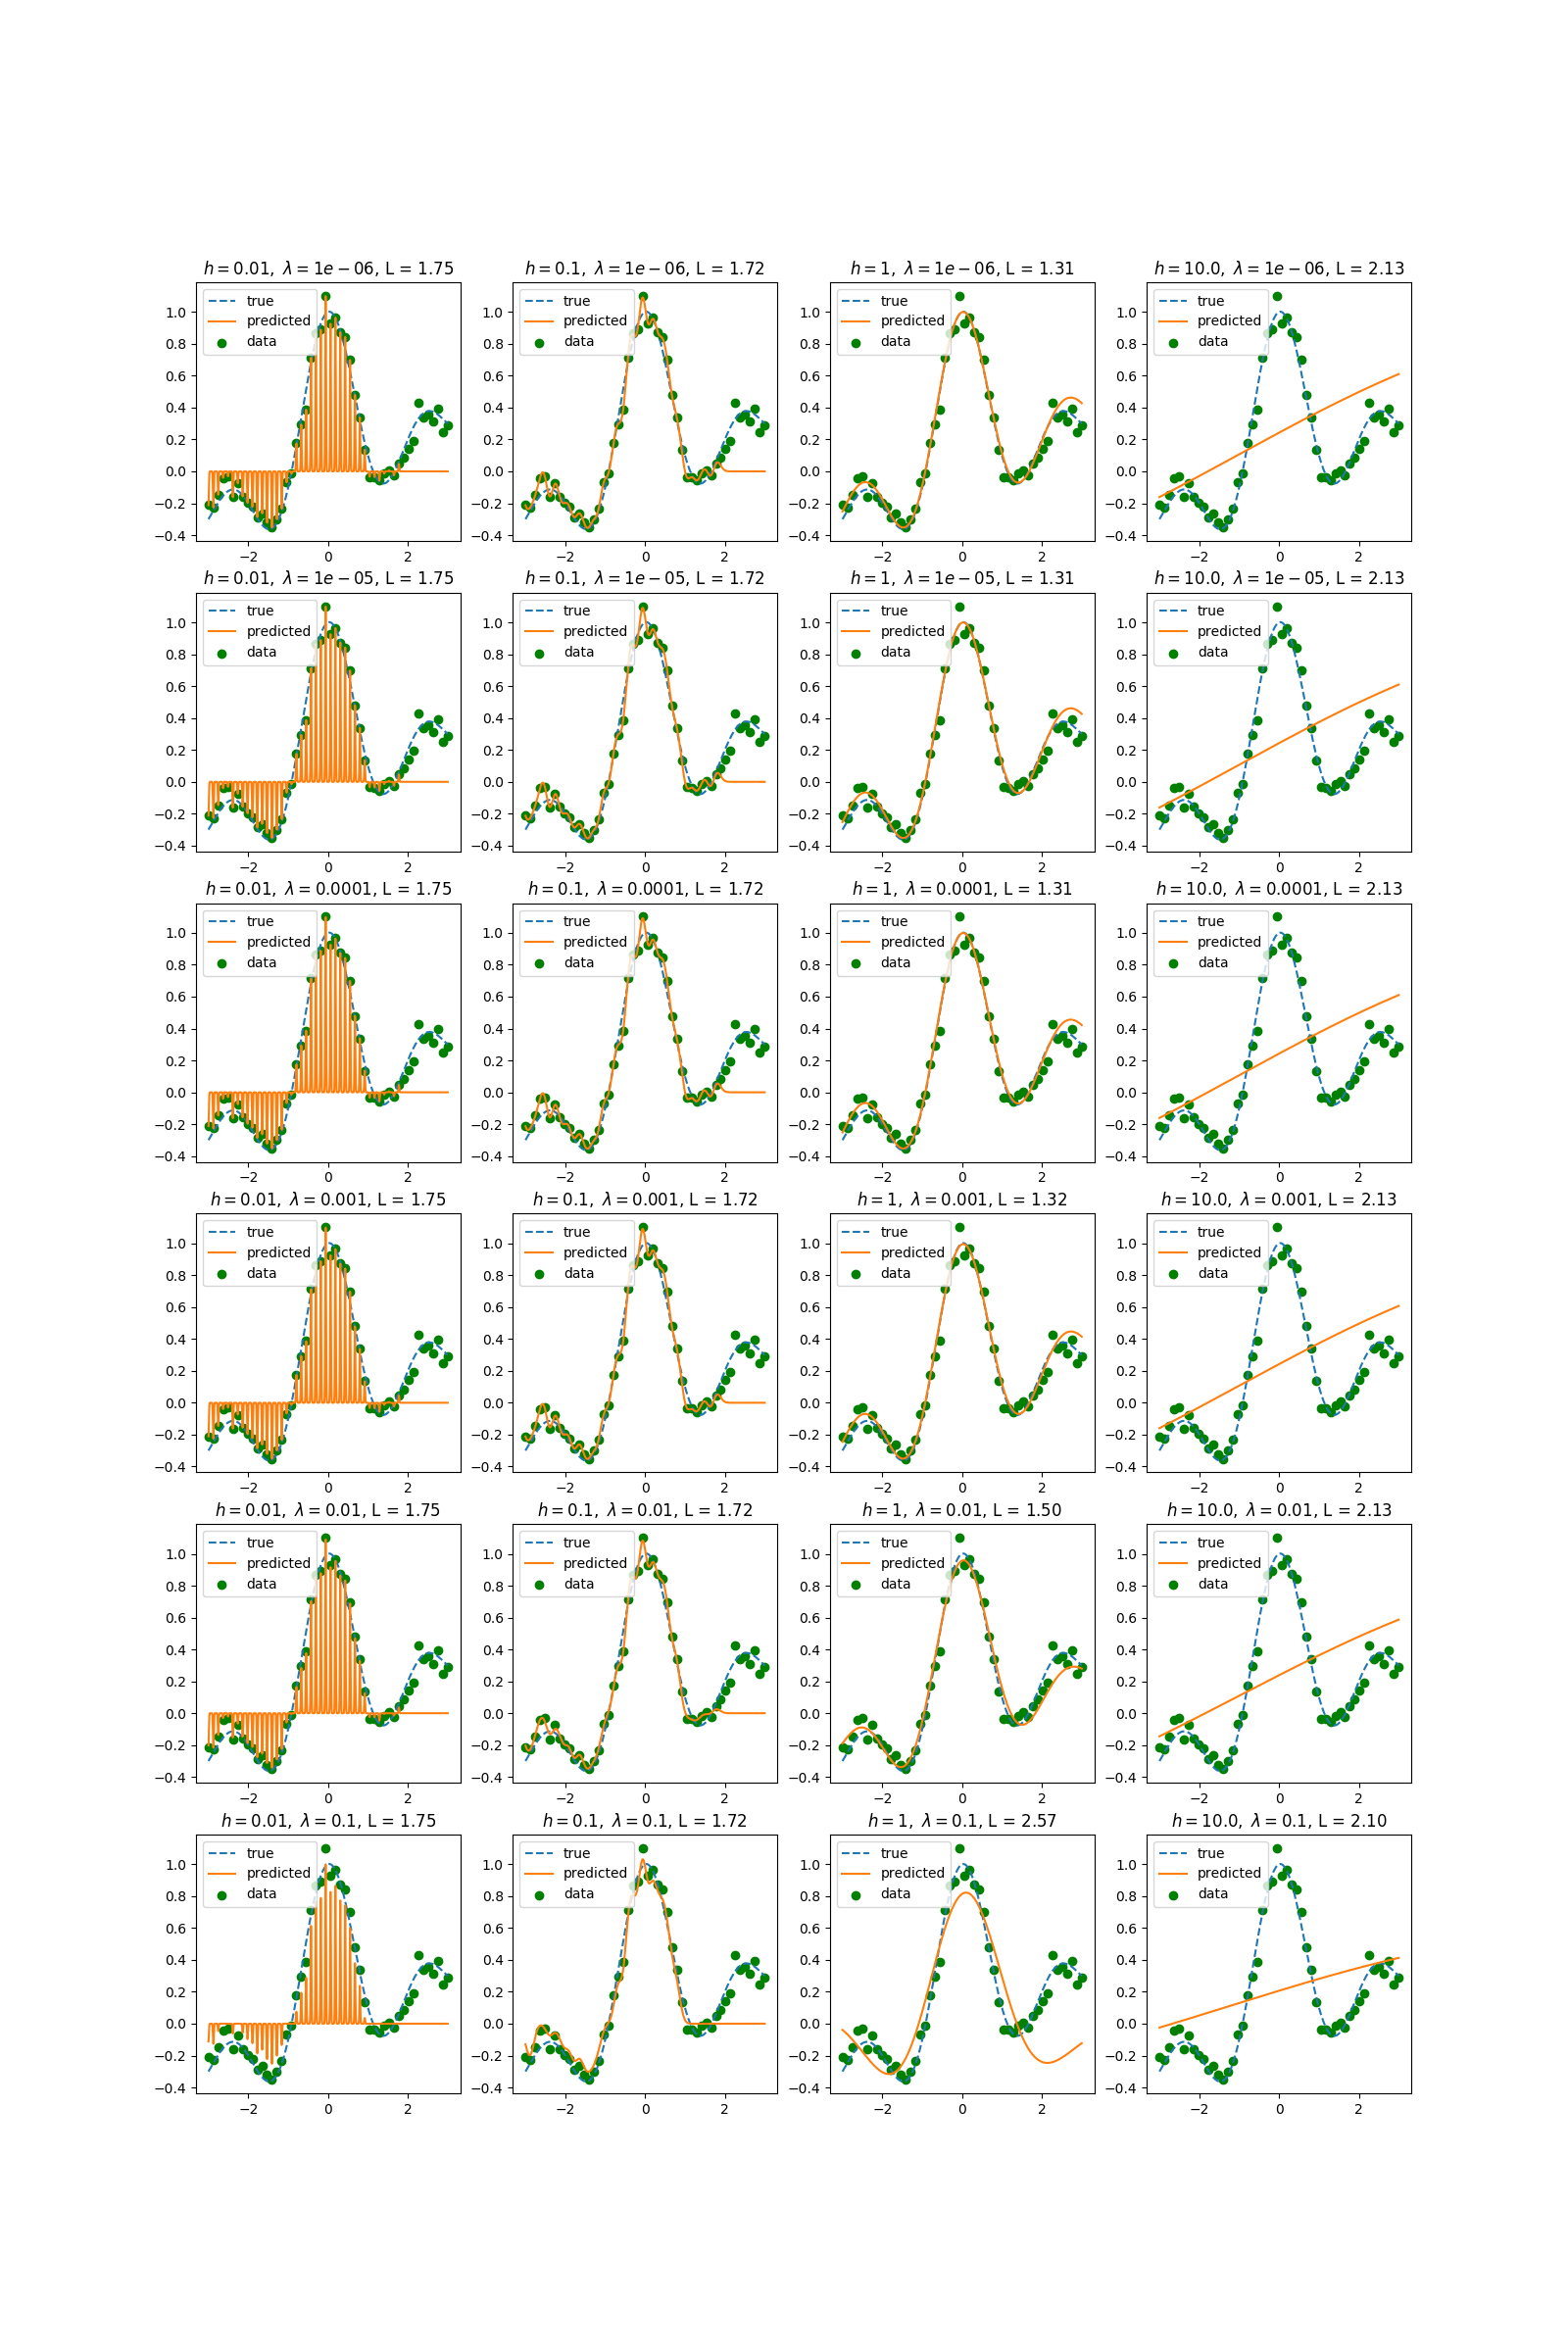
\includegraphics[clip, width=15cm, trim=0 144 0 216]{../figures/assignment2_result}
	\caption{交差確認法の結果}
	\label{fig:result_global_search}
\end{figure}



\end{document}
